\begin{qunlist}


\q{$\bigstar\bigstar$}{Minimal Positive Valued Function}

Consider a strictly decreasing function $f :
\mathbb{N} \rightarrow \mathbb{Z}$, such that $f(i) > f(i + 1)$ for all $i \in \mathbb{N}$. Assuming we can evaluate $f$ at any number in constant time, we want to find $n = \min\{i \in \mathbb{N}:f(i) < 0\}$. Design a $O(\log n)$ algorithm to compute $n$.

\textit{(Please turn in a four part solution to this problem.)}\\
\answer{\\
\textbf{Main Idea}\\
Keep doubling an index $i$ starting at one until $f(i)<0$. Once a nonzero element is reached, then you know that $n = \min\{i \in \mathbb{N}:f(i) < 0\} \in (\frac{i}{2}, i]$. Then, run a slightly modified binary search on that interval. \\
\textbf{Pseudocode}\\
minIndex(f)\\
\tab $i=1$\\
\tab while $f(i)<0$\\
\tab \tab $i*=2$\\
\tab bSearch(i)\\ \\
bSearch(i)\\
\tab $\text{middle}=\frac{\frac{i}{2}+i}{2}$\\
\tab if $\text{f(middle)}<0$ AND $\text{f(middle-1)}\geq0$\\
\tab \tab return middle\\
\tab else if $\text{f(middle)}<0$\\
\tab \tab return bSearch(middle)\\
\tab else \\
\tab \tab return bSearch(middle$+\frac{i-\text{middle}}{2}$)\\
\textbf{Proof of Correctness}\\
If we stop the doubling of $i$ due to $f(i)<0$, then we know for sure that $f(\frac{i}{2}) \geq 0$. Then, it is clear that $\min\{i \in \mathbb{N}:f(i) < 0\} \in (\frac{i}{2}, i]$. We now reduce the problem to finding the first nonzero element in a "decreasing array" that has the elements $[f(\frac{i}{2})+1...,f(i-3),f(i-2),f(i-1),f(i)]$. Note that $i=2^k,k\in\mathbb{N}$. Then, a simple modification of binary search where the index limits are shifted, and the test for going to the left or right comes from whether or not $f(\text{middle})<0$ completes the algorithm.\\
\textbf{Running Time}\\
$O(\log(n))$\\
\textbf{Justification}\\
It will take at most $\ceil{\log_2(n)}$ doublings in order for $i$ to surpass $n$, the assumed first index where $f(n)<0$. Then, running binary search on an "array"(function evaluations are constant, so we can treat it like an array in terms of runtime) takes $O(\log(2^{\ceil{\log_2(n)}}-2^{\ceil{\log_2(n)}-1})) \in O(\log(n))$. The latter is the same as the former, so the overall runtime is simply $O(\log(n))$.
}


\pagebreak

\q{$\bigstar\bigstar$}{Graph Basics}

For parts (a) and (b), refer to the figure below. For parts (c) through (f), please prove only for simple graphs; that is, graphs that do not have any parallel edges or self-loops.

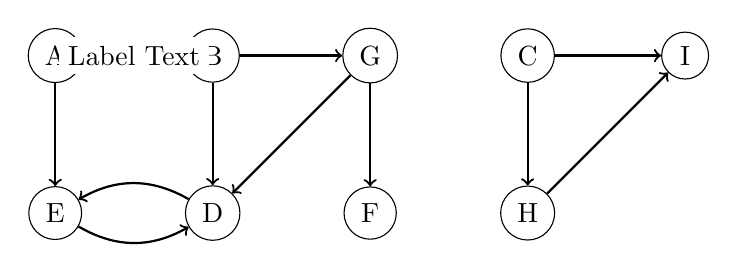
\begin{tikzpicture}
[ar/.style={->,thick},no/.style={draw,circle}]
\node [no] at (0cm,4cm) (A) {A};
\node [no] at (2cm,4cm) (B) {B};
\node [no] at (6cm,4cm) (C) {C};
\node [no] at (2cm,2cm) (D) {D};
\node [no] at (0cm,2cm) (E) {E};
\node [no] at (4cm,2cm) (F) {F};
\node [no] at (4cm,4cm) (G) {G};
\node [no] at (6cm,2cm) (H) {H};
\node [no] at (8cm,4cm) (I) {I};

\draw [ar] (A) -- (B) node [midway, fill=white] {Label Text};
\draw [ar] (A) -- (E);
\draw [ar] (B) -- (G);
\draw [ar] (G) -- (D);
\draw [ar] (B) -- (D);
\draw [ar] (D) to [bend right] (E);
\draw [ar] (E) to [bend right] (D);
\draw [ar] (G) -- (F);
\draw [ar] (C) -- (H);
\draw [ar] (C) -- (I);
\draw [ar] (H) -- (I);
\end{tikzpicture}

\begin{qparts}
\item Run DFS at node A, trying to visit nodes alphabetically (e.g. given a choice between nodes D and F, visit D first).

\begin{itemize}
\item List the nodes in the order you visit them (so each node should appear in the ordering exactly once).\\
\answer{
A,B,D,G,F,E,C,H,I
}
\item List each node with its pre- and post-number. The numbering starts from 1 and ends at 18.
\answer{
\begin{center}
	\begin{tabular}{ c c c c c c c c c c }
		 & A & B & C & D & E & F & G & H & I\\ 
		Pre &1&2&13&3&4&8&7&14&15 \\  
		Post &12&11&18&6&5&9&10&17&16     
	\end{tabular}
\end{center}
}
\item Label each edge as \textbf{T}ree, \textbf{B}ack, \textbf{F}orward or \textbf{C}ross.
\\
\answer{\\
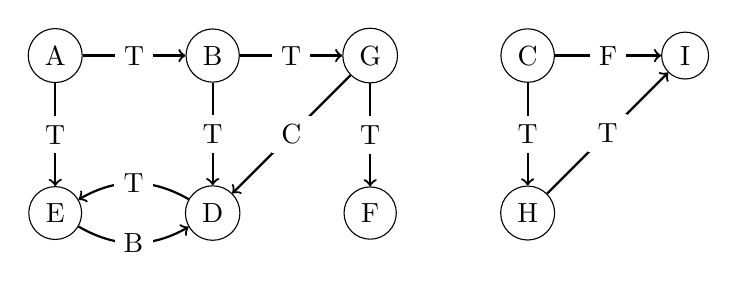
\begin{tikzpicture}
[ar/.style={->,thick},no/.style={draw,circle}]
\node [no] at (0cm,4cm) (A) {A};
\node [no] at (2cm,4cm) (B) {B};
\node [no] at (6cm,4cm) (C) {C};
\node [no] at (2cm,2cm) (D) {D};
\node [no] at (0cm,2cm) (E) {E};
\node [no] at (4cm,2cm) (F) {F};
\node [no] at (4cm,4cm) (G) {G};
\node [no] at (6cm,2cm) (H) {H};
\node [no] at (8cm,4cm) (I) {I};

\draw [ar] (A) -- (B) node [midway, fill=white] {T};
\draw [ar] (A) -- (E) node [midway, fill=white] {T};
\draw [ar] (B) -- (G) node [midway, fill=white] {T};
\draw [ar] (G) -- (D) node [midway, fill=white] {C};
\draw [ar] (B) -- (D) node [midway, fill=white] {T};
\draw [ar] (D) to [bend right] node[midway, fill=white] {T} (E);
\draw [ar] (E) to [bend right] node[midway, fill=white] {B} (D);
\draw [ar] (G) -- (F) node [midway, fill=white] {T};
\draw [ar] (C) -- (H) node [midway, fill=white] {T};
\draw [ar] (C) -- (I) node [midway, fill=white] {F};
\draw [ar] (H) -- (I) node [midway, fill=white] {T};
\end{tikzpicture}
}
\end{itemize}


\item Let $|E|$ be the number of edges in a simple graph and $|V|$ be the number of vertices. Show that $|E|$ is in $O(|V|^2).$
\answer{
Saw we have $|V|$ vertices. Then to maximize $|E|$ we should make our graph complete. That is, $|V|$ is connected to every other vertex possible. Then, we have that the first vertex can connect to $|V|-1$ other vertices, and the second vertex can connect to $|V|-2$ vertices, and so forth. So the total number of edges is 
$$\sum_{i=0}^{|V|}i \in O(|V|^2)$$ \qed
}


\item For each vertex $v_i$, let $d_i$ be the \textit{degree}- the number of edges incident to it. Show that $\sum d_i$ must be even. 
\answer{\\
Proof by induction on $|V|$.\\
Base case: $|V|=1\Rightarrow\sum d_i=0$.\\
Inductive Hypothesis: If a graph with $|V|$ vertices has $\sum d_i$ even, then any graph with $|V|+1$ must also have $\sum d_i$ even.\\
Inductive Step: To avoid build-up error, instead of adding a vertex to achieve a graph of $|V|+1$ vertices, we assume that we have any arbitrary graph with $|V|+1$ vertices. Now, remove any vertex, and the inductive hypothesis now applies to the new graph. This is valid because we do not require our graph to be connected. Now, after replacing the node that we removed, we can see that any edge that was nullified due to the removal that comes back adds 2 to $\sum d_i$. Thus, any amount of edges nullified that are restored can only change $\sum d_i$ by a multiple of 2, maintaining the evenness. \qed 
}



\end{qparts}

\pagebreak


\q{$\bigstar\bigstar\bigstar$}{Peak element} \\
Prof. Garg just moved to Berkeley and would like to buy a house with a view on Euclid Ave. 
Needless to say, there are $n$ houses on Euclid Ave, they are arranged in a single row, and have distinct heights. 
A house ``has a view'' if it is taller than its neighbors. 
For example, if the houses heights were $[3, 7, 5, 9]$, then $7$ and $9$ would ``have a view''.

Devise an efficient algorithm to help Prof. Garg find a house with a view on Euclid Ave. 
(If there are multiple such houses, you may return any of them.)\\
\answer{\\
\textbf{Main Idea}\\Looking at the middle element of the array, we can determine whether or not there is a "peak" in the left, right, or both of the left and right subarrays, or, if the middle element is a peak itself. This splits the problem in half. \\
\textbf{Pseudocode}\\
findPeak(houses)\\
$\text{middle}=\frac{\text{size(houses)}}{2}$\\
\tab if size(houses) $==$ 1 \\
\tab \tab return houses[0] \\
\tab if size(houses) $==$ 2 \\
\tab \tab return larger of two \\
\tab if $\text{houses(middle)}<houses(middle+1)$\\
\tab \tab return findPeak(houses[middle:]) \\
\tab else if $\text{houses(middle)}<houses(middle-1)$\\
\tab \tab return findPeak(houses[:middle])\\
\tab else return houses[middle] \\
\textbf{Proof of Correctness} \\
If $\text{houses(middle)}<houses(middle+1)$, then there are two cases:
\begin{enumerate}
	\item The second half of the houses array is strictly increasing. Then the last house must be a peak. 
	\item The second half of the houses array is not strictly increasing, meaning that somewhere, there must be at least one "turning point" where the houses start to decrease. The "turning point" must then be a peak.
\end{enumerate}
If $\text{houses(middle)}>houses(middle+1)$, then there are two cases:
\begin{enumerate}
	\item The first half of the houses array is strictly decreasing starting from the left. Then the first house must be a peak. 
	\item The second half of the houses array is not strictly decreasing, meaning that somewhere, there must be at least one "turning point" where the houses start to increase. The "turning point" must then be a peak.
\end{enumerate}
If neither of the previous two cases are true, then the middle must be a peak. This proves that cutting the problem in half in this way is valid. \\
\textbf{Running Time}\\
$O(log(n))$\\
\textbf{Justification}\\
At each stage, we are eliminating one half of the array, halving the problem size.
}
 

\pagebreak

\q{$\bigstar\bigstar\bigstar$}{Exact Change}

Your friend from Mars visits you and wants to buy a CS 170 textbook, which is priced at $\$t$ dollars. Unfortunately, Martians have their own currency. You are given an array $A[0..n-1]$ with $n$ elements representing the value of each Martian coin in dollars. The value of each coin is a distinct integer in the range $0 \le A[i] \le 170n$. For some reason, your friend brought only 4 coins of each type. 

Design an efficient algorithm that determines, given $A$ and $t$, whether your friend can give you exact change. Note: the algorithm should run asymptotically faster than $O(n^2)$.

\textit{(Please turn in a four part solution to this problem.)}\\
\textit{Hint: Think about properties of exponents.}\\
\answer{\\
\textbf{Main Idea}\\
Represent array A as a degree at most $170n$ polynomial. 
$$p(x)=a_0+a_1x^1+a_2x^2+...+a_{170n}x^{170n}, a_0=1$$ 
Have the coefficient $a_i$ is either 1 or 0 depending on if that element exists in $A$. Then, we can simply take this polynomial to the fourth power, and check to see if the result has a non-zero coefficient for the $n^t$ term, using FFT to do the heavy lifting of multiplying the polynomials.\\
\textbf{Pseudocode}\\
exactChange(DENOMS, COST)\\
\tab $\text{denomTuple}=\text{Coefficient representation of degree at most 170n polynomial of the form}\sum_{i=0}^{170n}a_ix^{A[i]}$\\
\tab $\text{valueDenomTuple}=\text{FFT evaluation performed on denomTuple}$\\
\tab Take the fourth power of each element in valueDenomTuple\\
\tab $\text{resultTuple}=\text{FFT interpolation on valueDenomTuple}$ \\
\tab if (resultTuple has nonzero coefficient for the $x^t$ term) \\
\tab \tab return true\\
\tab else \\
\tab \tab return false\\
\textbf{Proof of Correctness}\\
After the first squaring of $p(x)$, we have all the possible values that are possible with two coins of any two denominations. This is because of the nature of polynomial multiplication. Because the $x^c$ term represents a coin value of $c$, when multiplied with say $x^d$, we have $x^cx^d=x^{c+d}$, which gives us a term that corresponds to a value $c+d$ coin, as desired. Each term in the polynomial is multiplied with each of the other terms in the polynomial, including itself. The result must then be all the possible sums of two coins from the denomination list. Because we require four coins, we take the fourth power of $p(x)$.\\
\textbf{Running Time}\\
$O(n\log(n))$\\
\textbf{Justification}\\
Converting A to the coefficient representation of $p(x)$ takes $n$ time. Using FFT to evaluate a degree $170n$ polynomial takes time $170n\log(170n)$. However, we want to evaluate $p(x)$ at $4(170n)+1$ points, because we know that our result is of at most degree $680n$. This takes $680n\log(680n)$. Then, determining whether our desired term is in the result takes $n$ time. $O(2n+680n\log(680n)) \in O(n\log(n))$.
}




\pagebreak
\q{$\bigstar\bigstar\bigstar\bigstar$}{Local Maxima}

Consider an $n\times n$ matrix $M$ with distinct integer entries. Call an entry $M_{ij}$ a \emph{local maximum} if it is greater than all of its neighbors. More precisely, $M_{ij}$ is a local maximum if for all $a,b$ with $|i-a|\le 1$ and $|j-b|\le 1$, $M_{ij} \ge M_{ab}$. In an array $A$, say that $A_i$ is a \emph{local maximum} of $A$ is $A_i \ge A_{i+1}$ and $A_i \ge A_{i-1}$. Note that if $i$ is the last element in $A$, then $A_i \geq A_{i-1}$ is sufficient for $A_i$ to be local maximum, and similarly if $i$ is the first element, then $A_i \geq A_{i+1}$ is sufficient.

Suppose that $M$ is guaranteed to have exactly one local maximum and that every column of $M$, when viewed as an array, contains exactly one local maximum. Show that the local maximum of $M$ can be found in $O(\log^2 n)$ time. 

\text{(Please give a four part solution for this problem.)}



\pagebreak
\q{$\bigstar\bigstar\bigstar\bigstar\bigstar$}{DNA Sequence Alignment}

We are given binary strings $s,t$; $s$ is $m$ bits long, and $t$ is $n$ bits long,
and $m<n$.
We are also given an integer $k$.
We want to find whether $s$ occurs as a substring of $t$,
but with $\le k$ errors, and if so, find all such matches.
In other words, we want to determine whether there exists an index $i$
such that $s_0,s_1,\dots,s_{m-1}$ agrees with
$t_i,t_{i+1},t_{i+2},\dots,t_{i+m-1}$ in all but $k$ bits; and if yes,
find all such indices $i$.
\begin{qparts}
\item Describe an $O(mn)$ time algorithm for this string matching problem.
Just show the pseudocode; you don't need to give a proof of correctness
or show the running time.\\
\answer{\\
	\textbf{Pseudocode}\\
	stringMatch(s,t,k)\\
	\tab $\text{result}=[]$\\
	\tab $\text{tCounter}=0$\\
	\tab while($\text{tCounter}<\text{len(t)}-\text{len(s)}$)\\
	\tab \tab if length $s$ array starting at tCounter has $\leq k$ errors.\\
	\tab \tab \tab append tCounter to result\\
	\tab \tab $\text{tCounter}+=1$
}

\item Let's work towards a faster algorithm.
Suggest a way to choose polynomials $p(x),q(x)$ of degree $m-1,n-1$,
respectively, with the following property:
the coefficient of $x^{m-1+i}$ in $p(x)q(x)$ is $m-2d(i)$,
where $d(i)$ is the number of bits that differ between
$s_0,s_1,\dots,s_{m-1}$ and $t_i,t_{i+1},t_{i+2},\dots,t_{i+m-1}$.

Hint: use coefficients $+1$ and $-1$.

\item Describe an $O(n \lg n)$ time algorithm for this string matching problem,
taking advantage of the polynomials $p(x),q(x)$ from part (b).

\item Now imagine that $s,t$ are not binary strings, but DNA sequences:
each position is either A, C, G, or T (rather than 0 or 1).
As before, we want to check whether $s$ matches any substring of $t$
with $\le k$ errors
(i.e., $s_0,s_1,\dots,s_{m-1}$ agrees with
$t_i,t_{i+1},t_{i+2},\dots,t_{i+m-1}$ in all but $k$ letters),
and if so, output the location of all such matches.
Describe an $O(n \lg n)$ time algorithm for this problem.

Hint: encode each letter into 4 bits.


\end{qparts}


\pagebreak
\q{$???$}{(Optional) Redemption for Homework 1}

Submit your \emph{redemption file} for Homework 1 on Gradescope. If you looked at the solutions and took notes on what you learned or what you got wrong, include them in the redemption file. 


\end{qunlist}
